%% 
%% Copyright 2007, 2008, 2009 Elsevier Ltd
%% 
%% This file is part of the 'Elsarticle Bundle'.
%% ---------------------------------------------
%% 
%% It may be distributed under the conditions of the LaTeX Project Public
%% License, either version 1.2 of this license or (at your option) any
%% later version.  The latest version of this license is in
%%    http://www.latex-project.org/lppl.txt
%% and version 1.2 or later is part of all distributions of LaTeX
%% version 1999/12/01 or later.
%% 
%% The list of all files belonging to the 'Elsarticle Bundle' is
%% given in the file `manifest.txt'.
%% 
%% Template article for Elsevier's document class `elsarticle'
%% with harvard style bibliographic references
%% SP 2008/03/01

\documentclass[preprint,12pt,authoryear]{elsarticle}

%% Use the option review to obtain double line spacing
%% \documentclass[authoryear,preprint,review,12pt]{elsarticle}

%% Use the options 1p,twocolumn; 3p; 3p,twocolumn; 5p; or 5p,twocolumn
%% for a journal layout:
%% \documentclass[final,1p,times,authoryear]{elsarticle}
%% \documentclass[final,1p,times,twocolumn,authoryear]{elsarticle}
%% \documentclass[final,3p,times,authoryear]{elsarticle}
%% \documentclass[final,3p,times,twocolumn,authoryear]{elsarticle}
%% \documentclass[final,5p,times,authoryear]{elsarticle}
%% \documentclass[final,5p,times,twocolumn,authoryear]{elsarticle}

%% For including Fig.s, graphicx.sty has been loaded in
%% elsarticle.cls. If you prefer to use the old commands
%% please give \usepackage{epsfig}

%% The amssymb package provides various useful mathematical symbols
\usepackage{amssymb}
%% The amsthm package provides extended theorem environments
%% \usepackage{amsthm}
\usepackage{amsmath}

\usepackage[
  breaklinks=true,
  colorlinks=true,
  linkcolor=blue,anchorcolor=blue,
  citecolor=blue,filecolor=blue,
  menucolor=blue,pagecolor=blue,
  urlcolor=blue]{hyperref}

% Let's add todonotes and comments:
\usepackage[draft]{todonotes}

% Select what to do with command \comment:  
% \newcommand{\comment}[1]{}  %comment not showed
\newcommand{\comment}[1]
{{[\bfseries \color{blue} #1]}} %comment showed

%% The lineno packages adds line numbers. Start line numbering with
%% \begin{line numbers}, end it with \end{linenumbers}. Or switch it on
%% for the whole article with \linenumbers.
\usepackage{lineno}
\usepackage{float}
%\usepackage{wrapfig}
%\usepackage[backend=bibtex]{biblatex}  % to compile bib in R: http://texblog.org/2013/08/20/rknitr-automatic-bibliography-generation-with-biblatex-in-rstudio/
\usepackage[anythingbreaks]{breakurl}

\begin{document}

\begin{frontmatter}

%% Title, authors and addresses

%% use the tnoteref command within \title for footnotes;
%% use the tnotetext command for theassociated footnote;
%% use the fnref command within \author or \address for footnotes;
%% use the fntext command for theassociated footnote;
%% use the corref command within \author for corresponding author footnotes;
%% use the cortext command for theassociated footnote;
%% use the ead command for the email address,
%% and the form \ead[url] for the home page:
%% \title{Title\tnoteref{label1}}
%% \tnotetext[label1]{}
%% \author{Name\corref{cor1}\fnref{label2}}
%% \ead{email address}
%% \ead[url]{home page}
%% \fntext[label2]{}
%% \cortext[cor1]{}
%% \address{Address\fnref{label3}}
%% \fntext[label3]{}

\title{A platform for crowdsourcing the creation of representative, accurate landcover maps}

%% use optional labels to link authors explicitly to addresses:
%% \author[label1,label2]{}
%% \address[label1]{}
%% \address[label2]{}

\author[label1,label2]{Estes, L.D.\corref{cor1} \fnref{fn1}}
\ead{lestes@princeton.edu}
\author[label3]{McRitchie, D.\fnref{fn1}}
\author[label1]{Choi, J.}
\author[label1]{Debats, S.}
\author[label4]{Evans, T.}
\author[label1]{Guthe, W.}
\author[label1]{Luo, D.}
\author[label1]{Ragazzo, G.}
\author[label1]{Zempleni, R.}
\author[label1]{Caylor, K.K.}

\address[label1]{Civil and Environmental Engineering, Princeton University, Princeton, NJ, 08544 USA}
\address[label2]{Woodrow Wilson School, Princeton University, Princeton, NJ, 08544 USA}
\address[label3]{Computational Science and Engineering Support, Office of Information Technology, Princeton University, Princeton, NJ, 08544 USA}
\address[label4]{Department of Geography, Indiana University, Bloomington, IN 47405 USA}
\cortext[cor1]{Corresponding author}
\fntext[fn1]{Equal contributors}

\begin{abstract}
% Abstract header text removed in elsearticle.cls to allow highlights to be inserted. 
\textbf{Highlights}
\begin{itemize}
  \item DIYlandcover crowdsources the generation of landcover data, using human pattern recognition skill to create accurate maps with rich geometric detail.  
  \item It incorporates representative sampling and worker-specific accuracy assessment protocols, and connects to a large online job market. This design addresses three problems with crowdsourced mapping: representativity; data reliability; product delivery speed. 
  \item In a trial case, South African cropland was mapped with 91\% accuracy by novice workers. A scaling up analysis found that an Africa-wide cropland map could potentially be developed using this software for \$2-3 million within 1.2-3.8 years. 
\end{itemize}
\textbf{Abstract}\\
Accurate landcover maps are fundamental to understanding socio-economic and environmental patterns and processes, but existing datasets contain substantial errors. Crowdsourcing map creation may substantially improve accuracy, particularly for discrete cover types, but the quality and representativeness of crowdsourced data is hard to verify. We present an open-sourced platform, DIYlandcover, that serves representative samples of high resolution imagery to an online job market, where workers delineate individual landcover features of interest. Worker mapping skill is frequently assessed, providing estimates of overall map accuracy and a basis for performance-based payments. A trial of DIYlandcover showed that novice workers delineated South African cropland with 91\% accuracy, exceeding the accuracy of current generation global landcover products, while capturing important geometric data. A scaling-up assessment suggests the possibility of developing an Africa-wide vector-based dataset of croplands for \$2-3 million within 1.2-3.8 years. DIYlandcover can be readily adapted to map other discrete cover types.    
\end{abstract}
%% Text of abstract

\begin{keyword}
remote sensing \sep landcover \sep crowd-sourcing \sep accuracy assessment \sep representative sampling \sep object extraction
\end{keyword}


\end{frontmatter}


\linenumbers

\section*{Availability}
\indent DIYlandcover's source code will be made available free of charge for suitable non-commercial purposes under a GPLv3 license, upon consultation with the authors. For those interested in commercial applications, the prospective licensee should contact Princeton University's Office of Technology Licensing. The details of a specific application of the software for delineating crop fields in sub-Saharan Africa can be found at \\
\href{http://mappingafrica.princeton.edu}{mappingafrica.princeton.edu}, together with associated information about participating in the project, including digitizing rules and links for accessing the mapping interface.

%% main text
\section{Introduction}
Regional maps of landcover provide critical information on food security estimates \citep[e.g.][]{monfreda_farming_2008,licker_mind_2010,see_improved_2015,lobell_use_2013}, models of land-atmosphere interactions \citep[e.g.][]{liang_simple_1994}, and calculations of carbon stocks \citep[e.g.][]{ruesch_new_2008}, greenhouse gas emissions \citep[e.g.][]{searchinger_high_2015}, and habitat change \citep[e.g.][]{gibbs_tropical_2010}. These maps are particularly important in developing regions, such as sub-Saharan Africa, where government land use data are often lacking, error-prone, and inconsistent \citep{ramankutty_farming_2008,see_improved_2015}. These developing regions are also experiencing rapid land use changes \citep{gibbs_tropical_2010,rulli_global_2013} that pose pressing development challenges \citep[e.g. how to feed people at substantially lower environmental cost][]{searchinger_high_2015}. 

Unfortunately, landcover datasets derived from medium to coarse resolution satellite sensors are particularly inaccurate \citep{fritz_comparison_2010, fritz_identifying_2008}. One major reason for poor accuracy is the fact that land use patterns in these regions are dominated by smallholder farming. Smallholder fields are typically smaller ($\leq$2 ha) than the resolution ($\sim$6 ha) of the most commonly used satellite imagery \citep{jain_mapping_2013}. Furthermore, smallholders often plant diverse mixtures of crops, which further increases within-pixel heterogeneity \citep{jain_mapping_2013}, and their fields often contain remnant trees and have irregular boundaries, which makes them spectrally harder to distinguish from the surrounding vegetation \citep{see_improved_2015, lobell_use_2013}. 

New techniques for merging multiple landcover products are helping to substantially improve map accuracy \citep{fritz_cropland_2011,fritz_mapping_2015}. However, these approaches cannot overcome the mismatch between sensor resolution and smallholder field size. High resolution satellite imagery ($<$5 m) is becoming increasingly available--and presumably will become more affordable--so the resolution problem should be solved in the near future \citep{see_improved_2015, lobell_use_2013}. But high resolution comes at the expense of higher spectral variability; centimeter-scale data require lower orbits, narrower swaths, and greater communication bandwidth, which combine with clouds to greatly limit the area that can be imaged under contemporaneous environmental conditions, and from comparable viewing angles. This means that high resolution image mosaics covering large areas contain substantial and largely uncorrectable spectral differences caused by variations in atmospheric conditions, vegetation phenology, and bidirectional reflectance. This variability propagates error in automated classifications over large regions, which can already be substantial when there is high within-cover variability \citep{debats_generalized_2015}, or high heterogeneity among cover types \citep{gross_monitoring_2013}.  

%However, high spatial resolution typically comes at the cost of greater image variability; a meter-scale dataset requires satellites flying in Low Earth orbits, thus to cover wide areas it is typically necessary to piece together imagery acquired on different dates, by different sensors, pointing at different viewing angles. This resulting image quilt contains large and often uncorrectable spectral variability caused by atmospheric effects, vegetation phenology, variations in bidirectional reflectance, and even land use change. This variability propagates into classification error.  

It remains a major challenge to develop algorithms that can accurately classify landcover in the face of both increased image variability and substantial spatial heterogeneity. Promising methods are emerging, however, which draw on advances in computer vision and machine learning, such as semantic segmentation \citep[e.g.][]{schroff_object_2008} and Randomized Quasi-Exhaustive feature selection \citep{tokarczyk_features_2015}, to find optimal classifiers within complex urban environments \cite{frohlich_land_2013} and highly variable smallholder fields \citep[e.g.][]{debats_generalized_2015}. However, these advances are primarily in pixel-wise classification. Accurate, automated methods for extracting individual objects within a single cover type, particularly over wide areas, is arguably even more difficult. Object delineation is an important goal of landcover mapping, as cover geometries encode critical social and environmental information \citep{fritz_mapping_2015}, and can play an important role in improving environmental monitoring systems. For example, in agroecosystems, field boundaries can provide a filter for extracting ``pure'', crop-specific time series of satellite-derived vegetation indices, which helps to improve the accuracy of remotely sensed yield estimates \citep{estes_projected_2013, estes_comparing_2013}.  Some limited progress has been made with automated approaches, but these have been demonstrated mainly for small areas where the cover objects have regular geometries and sharp boundaries \citep[e.g. commercial agricultural fields][]{yan_automated_2014,ozdarici-ok_object-based_2014,ozdarici-ok_mapping_2015}. Such methods are not yet proven over large areas with more complex, less distinct cases. 

An alternative approach is to employ humans, who are very adept at recognizing patterns in noisy images \citep{biederman_recognition-by-components:_1987}. The superiority of human over machine pattern recognition provides the motivation for CAPTCHA \citep{ahn_captcha:_2003}, which secures websites by requiring human users to recognize fuzzy or irregular letters and numbers that are too difficult for automated algorithms to identify. Human-interpreted landcover maps are thus likely to be consistently more accurate than automated classifiers. Unfortunately, since humans are much slower at data processing than computers, human-generated landcover maps covering large areas will require much more time and expense to create. However, this problem is being alleviated by the growth of the internet, which makes it increasingly feasible to turn pattern recognition problems into many small tasks that are undertaken by a large number of online workers---the human equivalent of parallel processing. This ability to ``crowdsource'' \citep{howe_rise_2006} such work supports projects ranging from galactic classification \citep{lintott_galaxy_2008} to ornithological surveys \citep{sullivan_ebird:_2009}. Crowdsourcing of landcover is already being used in the Geo-wiki project, which uses online volunteers to correct landcover data based on their own interpretations of high resolution satellite imagery \citep{fritz_geo-wiki.org:_2009, fritz_geo-wiki:_2012, fritz_mapping_2015}. Recently, these data have been used to create the most accurate (82\%) global cropland map \citep{fritz_cropland_2011, fritz_mapping_2015}.  

While the use of crowdsourcing is an extremely promising development for landcover mapping, and is being increasingly used for this and other environmental monitoring applications \citep{jacobson_novel_2015,fraternali_putting_2012,schellekens_rapid_2014}, many existing projects (e.g. OpenStreetMap \href{openstreetmap.org}{(openstreetmap.org)}) are geared towards users who create content according to their personal interests, thus the resulting maps are unlikely to be geographically representative \citep{fraternali_putting_2012}. Furthermore, verifying the accuracy of crowdsourced data is a challenge \citep{allahbakhsh_quality_2013, flanagin_credibility_2008, see_improved_2015} that remains largely unaddressed by existing platforms. In terms of using crowdsourcing to improve landcover data, prior efforts have focused primarily on validating pixel-based classifications, and less on delineating individual cover objects, which is arguably one of the greatest advantages that people have over machines. Indeed, recognizing and digitizing individual, discrete cover types such as crop fields is considered fairly ``straightforward'' for humans \citep{yan_automated_2014}. 

%On top of this is the difficulty of segmentation, or object recognition, which is particularly important for discrete cover types, such as crop fields, where the geometries encode critical social and environmental characteristics of the land system \citep{fritz_mapping_2015}, and provide an important constraint for monitoring agroecosystems \citep[e.g][]{estes_projected_2013, estes_comparing_2013}. For example, field boundaries have been used as a filter to extract ``pure'', crop-specific time series of satellite-measured vegetation indices, allowing field-scale yield proxies to be derived \citep{estes_projected_2013, estes_comparing_2013}.  

In this paper, we describe \emph{\textbf{DIYlandcover}} (or ``Do-it-Yourself" landcover), a new platform for creating crowdsourced landcover data that addresses the three aforementioned limitations. DIYlandcover was designed for mapping discrete, but ``noisy'', cover types, where object extraction is of primary interest. Specifically, our platform provides online workers with tools to 1) delineate landcover objects within 2) representatively selected locations, while the resulting maps are subjected to 3) periodic quality assessments that provide estimates of individual worker and overall map accuracy. We provide an overview of DIYlandcover's design and mechanics, and report on the results of a trial application mapping crop fields in South Africa, which suggests that DIYlandcover allows inexperienced online workers to generate high accuracy ($>$90\%), geometrically rich, and geographically representative landcover data at a much faster rate than is usually possible with human-based mapping.

%On top of this is the difficulty of segmentation, or object recognition, which is particularly important for discrete cover types, such as crop fields, where the geometries encode critical social and environmental characteristics of the land system \citep{fritz_mapping_2015}, and provide an important constraint for monitoring agroecosystems \citep[e.g][]{estes_projected_2013, estes_comparing_2013}. For example, field boundaries have been used as a filter to extract ``pure'', crop-specific time series of satellite-measured vegetation indices, allowing field-scale yield proxies to be derived \citep{estes_projected_2013, estes_comparing_2013}.  


\section{System design}
The inspiration for DIYlandcover came from GeoTerraImage, a company that mapped South Africa's arable cropland by manually digitizing fields visible in high resolution satellite imagery  \citep{geoterraimage_south_2008}. The resulting map set is 97\% accurate in distinguishing cropped from uncropped areas at a 4 ha resolution (see detailed accuracy assessment in Appendix S1), and provides rich detail on field type and geometry. However, making these maps was an expensive and lengthy process; the estimated labor cost for digitizing was \$5 km$^{-2}$, and the project took approximately 2.5 years to complete (Ferreira, pers. comm.). 

We developed DIYlandcover to help overcome these constraints of cost and production time, while retaining the advantages of human image interpretation skill demonstrated by GeoTerraImage. Our platform connects workers in an online job marketplace to a map application programming interface (API) that hosts high resolution satellite imagery. DIYlandcover currently works with Amazon's Mechanical Turk \citep{amazon_web_services_amazon_2012} and the Google Maps API, but these could in principle be replaced by other services. These two aspects of DIYlandcover substantially reduce both mapping costs and completion times, because the imagery is free and the platform can access a potentially large number of workers. 

Given the distributed and anonymous nature of the online job market, we cannot intensively train workers (as GeoTerraImage did), yet our mapping task is complex, requires significant image interpretation skill, and must be completed in a systematic manner. Therefore, to ensure the scientific quality of its maps, DIYlandcover incorporates site selection and accuracy assessment protocols (Fig. 1). A sampling grid (SG in Fig. 1) over the desired study region provides the basis for collecting stratified random samples. The first draw identifies sites where the researcher/administrator \citep[the ``Requester'';][]{allahbakhsh_quality_2013} will provide landcover reference maps (black cells). Subsequent draws select sites where workers will create new maps (grey cells). This sample of locations is then sent to the job marketplace. All workers must pass an initial qualification test (Q1 in Fig. 1) that proves their ability to map a handful of sites with a minimum level of skill. Once qualified, workers begin mapping. Each worker will map both grey and black sites, which are respectively referred to as N (for normal) and Q (for quality assessment) sites. Q sites are indistinguishable from N sites, and are intermingled such that each worker has a Requester-defined probability of encountering a Q site. Completed maps from N sites are inserted into DIYlandcover's database (D), while maps from Q sites are first scored according to their agreement with their reference maps (Q2 in Fig. 1). Maps that fall below a minimum score are rejected. Map scores are incorporated into a worker-specific quality score, which is used to assign confidence to all maps generated by a worker, and to determine overall map accuracy. Workers are paid (P in Fig. 1) for each site mapped, with the possibility of bonus payments linked to quality scores.    

\begin{figure}[!ht]
  \begin{center}
    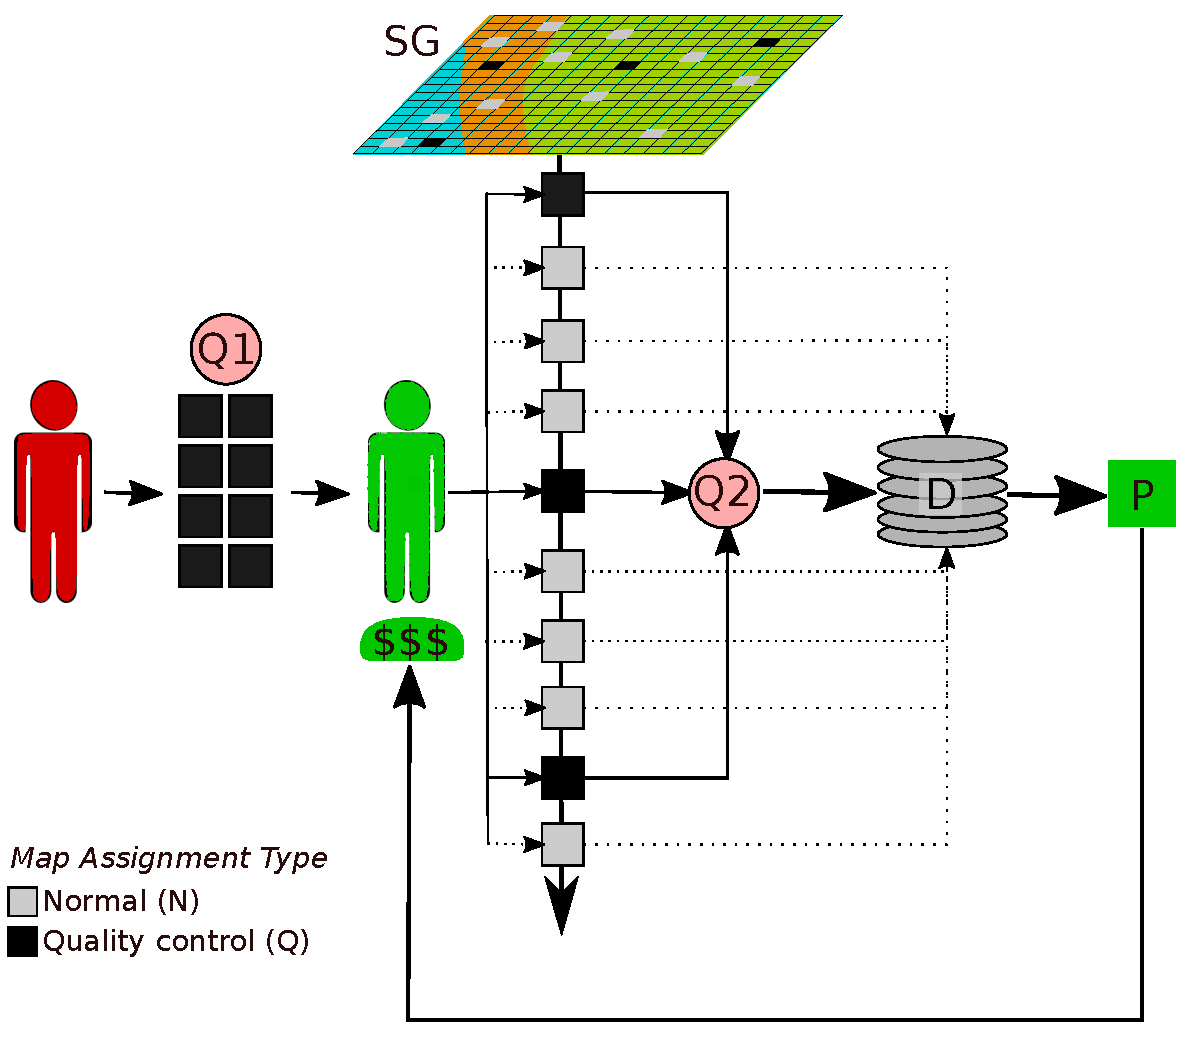
\includegraphics[scale=0.6]{fig1.eps}
    \caption{An overview of DIYlandcover's design. A survey grid (SG) is overlaid on a geographic area, and then random samples (weighted proportionally to the probability of cover type presence, represented by green, orange, and blue) are drawn to specify where groundtruth maps will be generated (black cells) to support worker map quality (Q) assessment. Subsequent random draws (grey cells) select sites that are undertaken as normal (N) mapping assignments. N and Q sites are sent inter-mingled to the online job marketplace for mapping. A first time worker (red) must take an initial map qualification test (Q1), after which she or he is qualified (green) and begins mapping. Maps from N sites are stored in the database (D); Q site maps are first scored based on their agreement with groundtruth (Q2). This score contributes to a longer term worker quality score, which is used to assess overall map quality and allows performance-based bonuses to be paid on of fixed per site payments (P).}
    \label{default}
  \end{center}
\end{figure}

\section{The mechanics of DIYlandcover}
The basic structure of DIYlandcover consists of three elements (Fig. 2): the main server hosting DIYlandcover's  database, here a Linux virtual machine with PostgresSQL (9.4) with the PostGIS (2.1) spatial extension;  a map server hosting the satellite imagery, in this case the Google Maps API \citep{google_developers_google_2012}; the online job market, Mechanical Turk \citep{amazon_web_services_amazon_2012}. Within this structure several key processes govern the creation and management of mapping tasks.  

\subsection{Site selection}
A ``master grid'' covering the study area is first created as a PostGIS table. Each cell provides a unique identifier, and the cell resolution defines the area of an individual mapping task. This grid is intersected with a second grid containing landcover occurrence probabilities, which are converted into categorical weights. A third field is created that indicates whether each cell is available to be mapped or not.  

%We use R \citep{r_development_core_team_r:_2011} and the raster \citep{etten_raster:_2011}, rgdal \citep{keitt_rgdal:_2012,warmerdam_geospatial_2008}, and rgeos \citep{bivand_rgeos:_2012} packages to generate the sampling grid, and then import it together with the probability grid into PostGIS where the intersection operations are performed.  

\begin{figure}[!ht]
  \begin{center}
       \makebox[\textwidth][c]{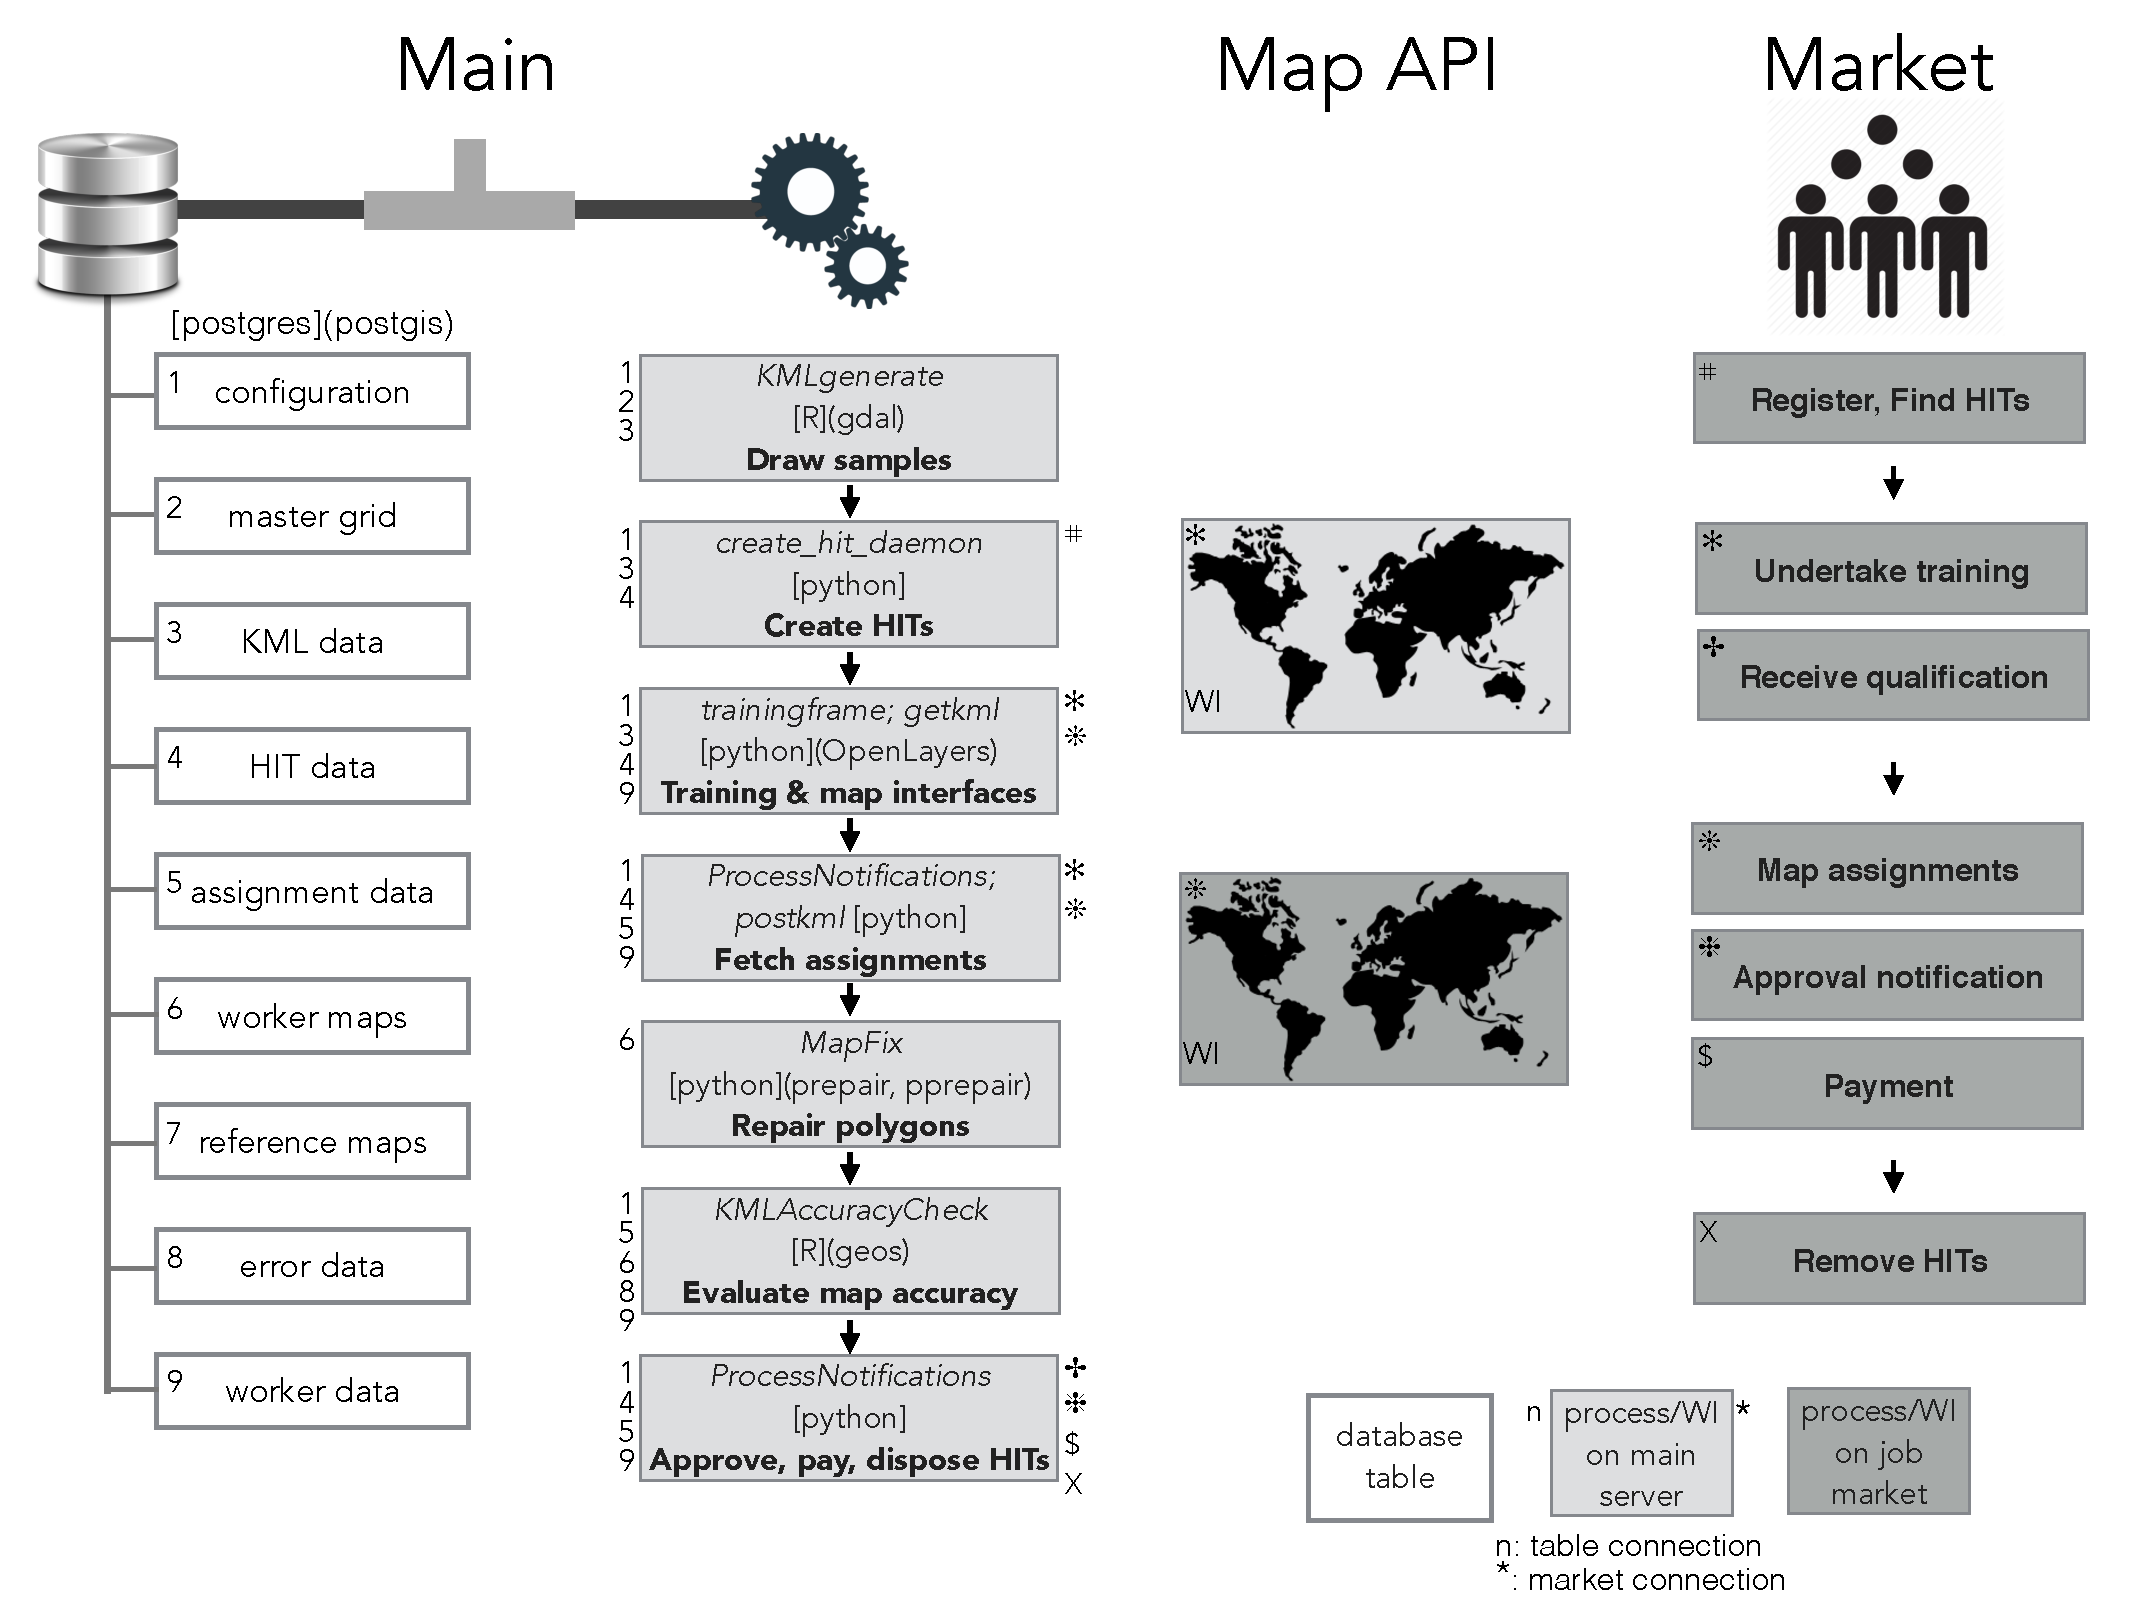
\includegraphics[width=1.3\textwidth]{fig2.eps}}
    %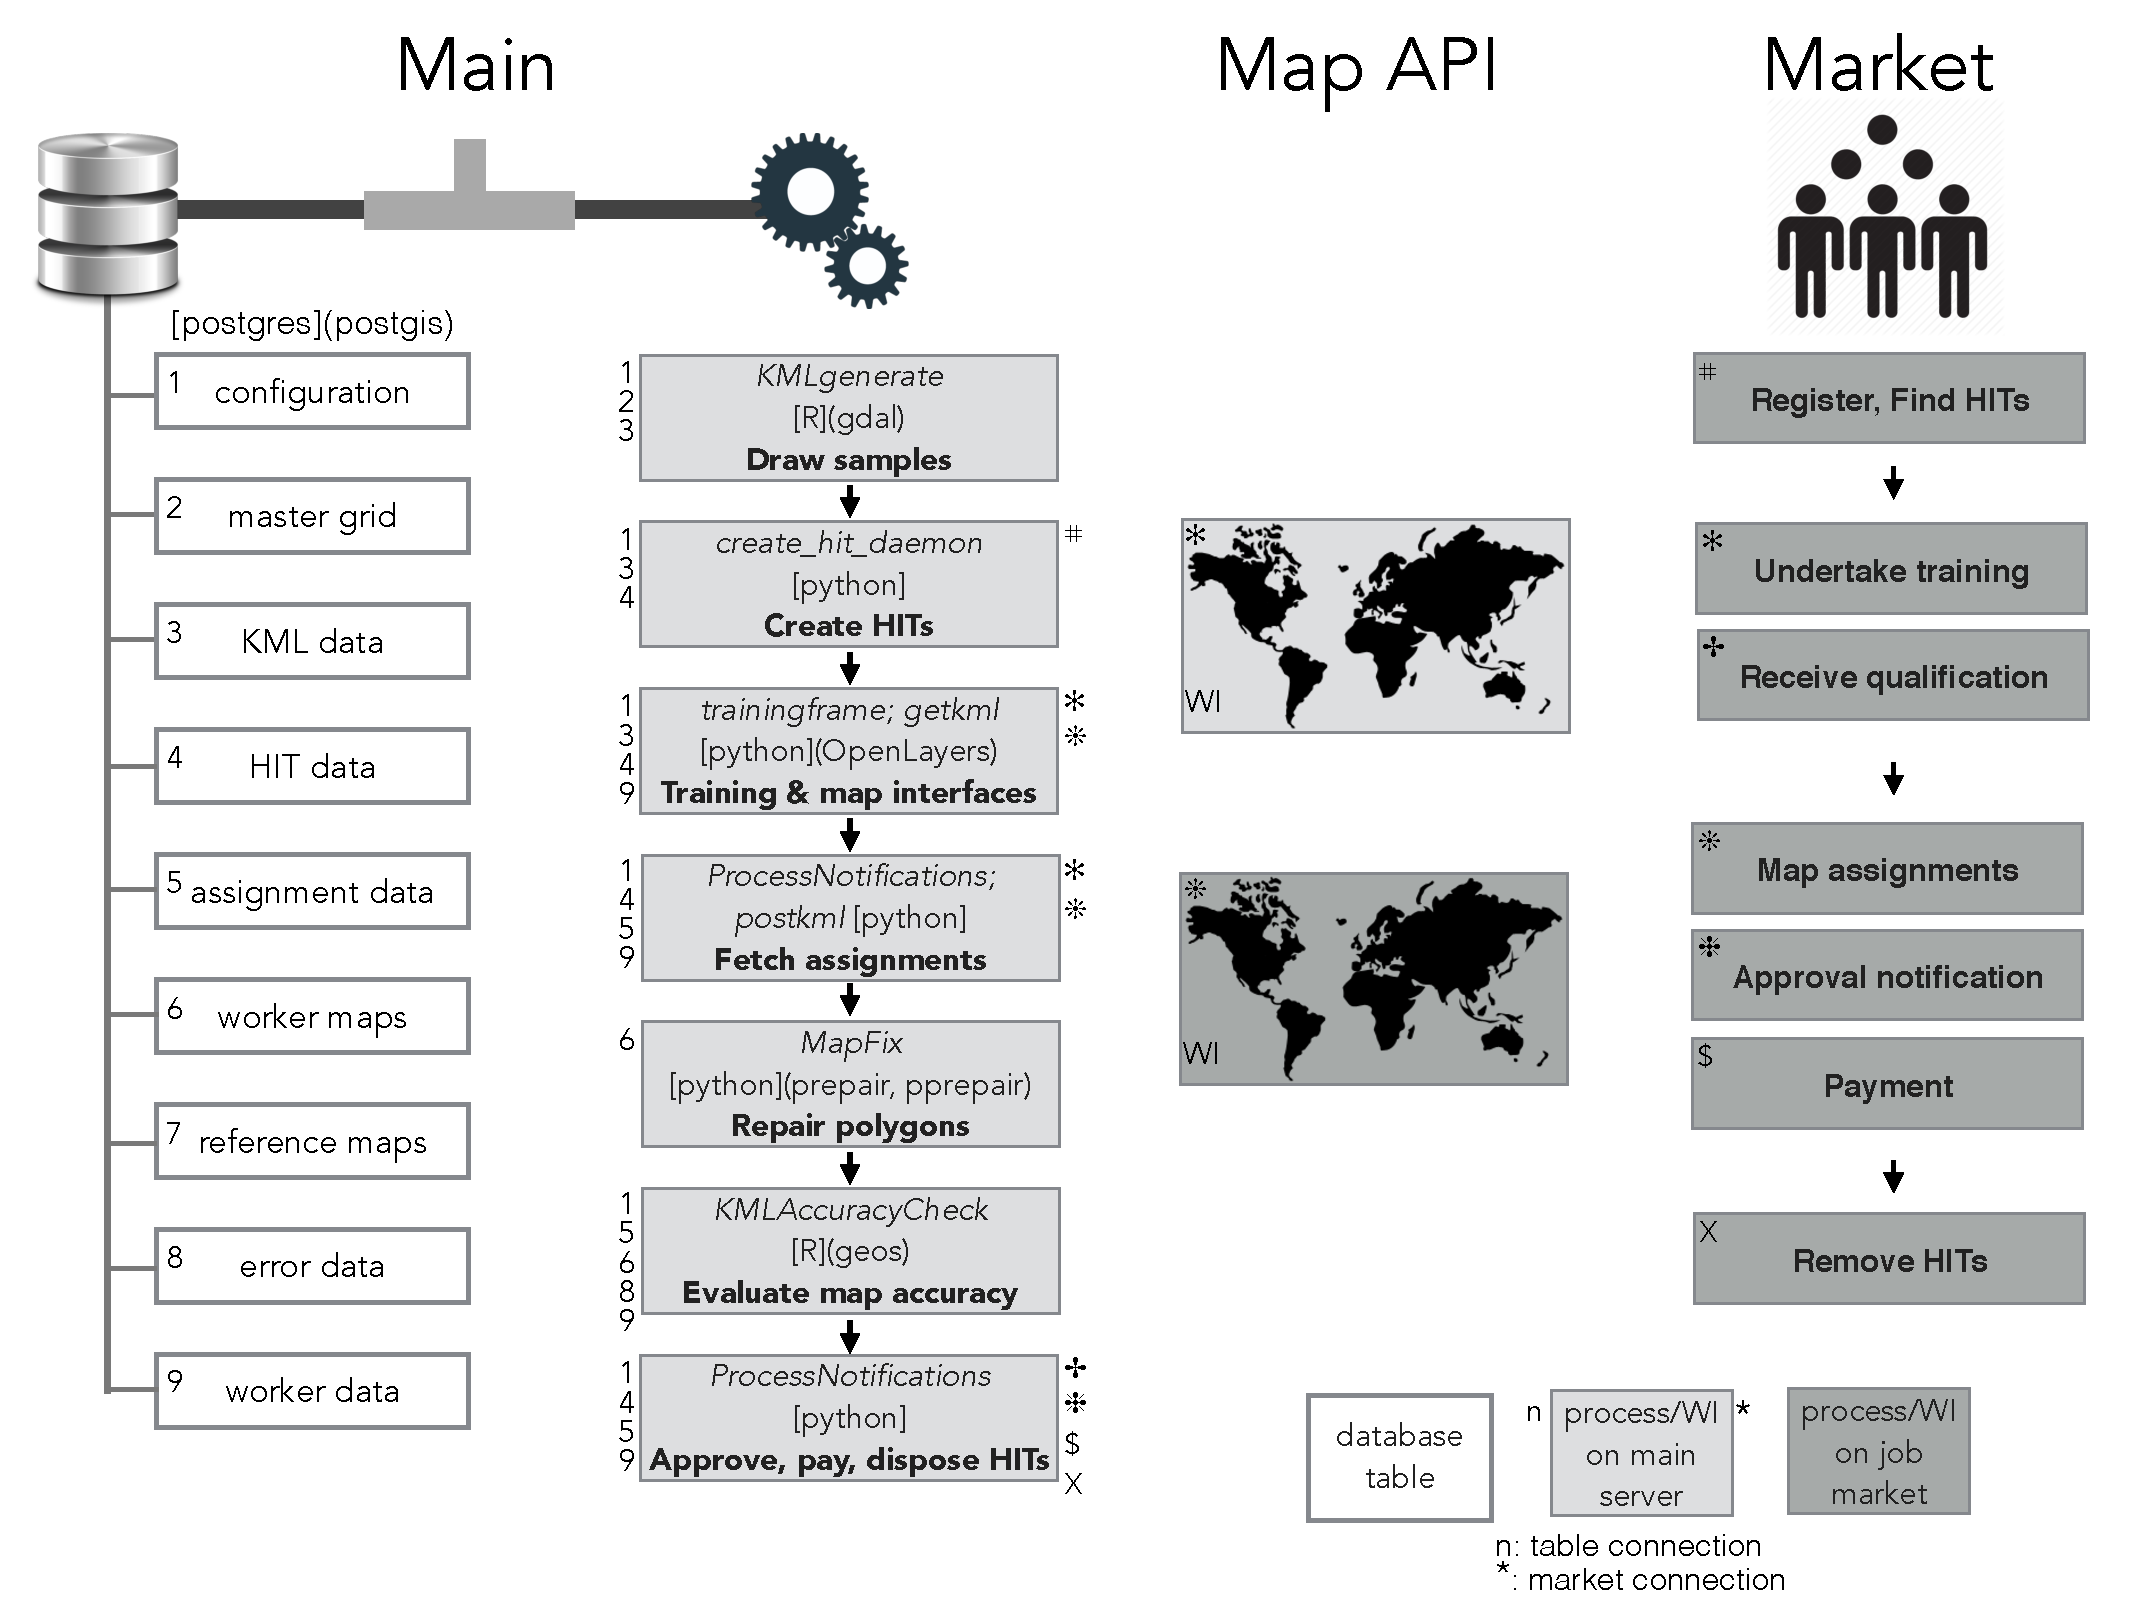
\includegraphics[scale=0.5]{fig2.eps}
    \caption{The components, and primary processes of DIYlandcover. The main server contains the system database and processes. Primary data tables are shown by the white boxes with grey borders. Primary processes are shown in light grey boxes (process names are italicized, primary software in brackets and its external dependencies in parenthesis, and description in bold). Server processes interact with specific data tables (indicated by the numbers to the left), and with processes that occur in the online job market (indicated by symbols to the right). The two versions (one for training, one for qualified workers) of the worker interface (WI) to the map API are shown, color-coded according to where they are hosted (on main server or online market). }
    \label{default}
  \end{center}
\end{figure}

After the initial random draw (of a user specified size) is taken to identify quality assessment (Q) sites (Section 2, Fig. 1), the selected cells' status is set to unavailable. The geometries are written to individual keyhole markup language (KML) files, and their IDs are added to a ``KML data'' table, where a field specifying cell type is set to "Q" to indicate that the corresponding KMLs reference quality control sites. The user has to provide landcover reference maps for these sites, the geometries of which are stored in a ``reference maps'' table.  

The next draw collects sites that will form the normal (``N'') map production process, where a worker (or workers) creates maps for locations where the underlying landcover is unknown.  This step is governed by \emph{KMLGenerate}, an R process that connects to the database \citep[via the RPostgreSQL package; ][]{conway_rpostgresql:_2012}, takes a weighted random draw of size X (a parameter stored in the ``configuration'' table that holds all variables used by DIYlandcover) from the master grid table, writes each cell geometry to a separate KML file, adds the selected cell IDs to the KML data table, and sets the field type value to ``N". The script changes the cell status in the master grid to unavailable. As N type maps assignments are completed, their status is set to mapped in the KML data table. \emph{KMLGenerate} runs as a daemon, selecting a new random draw as soon as the number of unmapped sites falls below a specified number, ensuring that there is never a system delay in sending mapping assignments to the job market (see 3.2).  

\subsection{Creating mapping assignments}
Following selection, each site is converted into a mapping task for online workers. These tasks are referred to as Human Intelligence Tasks (HITs), in Mechanical Turk's parlance. HITs are created by (\emph{create\_hit\_daemon}), a python daemon that uses the boto library to interface with Mechanical Turk (MT). The daemon polls MT (at regular intervals) to see how many DIYlandcover HITs of types Q and N exist on MT (zero at start of production), and whether they fall below their minimum required numbers. These numbers are calculated from two configuration parameters: the minimum total number of HITs that should be available on MT, and the percentage of these that should be of Q type. If the actual numbers of each type fall below their target numbers, \emph{create\_hit\_daemon} selects the IDs of available KMLs from the KML data table, and sends these together with associated HIT metadata, which includes the pay rate, the number of times the HIT should be mapped, the qualifications required to undertake the HIT (see 3.5), and a definition of the task. MT then registers each HIT and provides it with a unique HIT ID and registration time, which is logged into a ``HIT data'' table on the main server. 

\subsection{Undertaking the mapping assignment}
Once a HIT is registered on MT, it is visible to all workers in the marketplace, but can only be undertaken by qualified workers (see 3.5). Qualified workers who choose to undertake DIYlandcover-generated HITs are first shown a default HIT preview, and they must choose to accept it before they can see the actual location to map. This step helps prevent workers from declining more challenging sites, which bias the sample towards simpler landcovers.

To enable workers to perform a mapping HIT, DIYlandcover uses an OpenLayers interface to the image server, which sits within MT's user screen, centers the map view on the site of the HIT location, and provides a set of digitization tools  (Fig. 3). As soon as the worker accepts the HIT, it becomes a mapping assignment that is issued a unique assignment ID. A Web Server Gateway Interface (wsgi) script, \emph{getKML}, retrieves the OpenLayers javascript, the frame size parameters for the MT interface, the url for the KML demarcating the sample site, and user instructions (e.g. tool use tips), and passes these to MT, and collects the worker, assignment, and HIT IDs and acceptance time, and records these into the ``assignment data'' table. 

The worker then draws polygons around the landcover type(s) of interest that intersect the KML sample square (Fig. 3), and has the option to edit or delete individual geometries and provide comments. On completion, the worker saves the map, and is then taken to the next HIT preview screen. Alternatively, the worker may choose to return the assignment uncompleted. If this happens more than a specified number of times, the worker's qualification can be revoked (see 3.4), which is another check against sample selection bias.  The assignment is automatically abandoned if it is not completed within a defined time. We impose this last restriction to minimize bias in the estimation of wage rates (see 4.2); if workers leave the assignment unfinished on their computer for long periods, the amount of time required to complete assignments will be inflated.

\begin{figure}[!ht]
  \begin{center}
    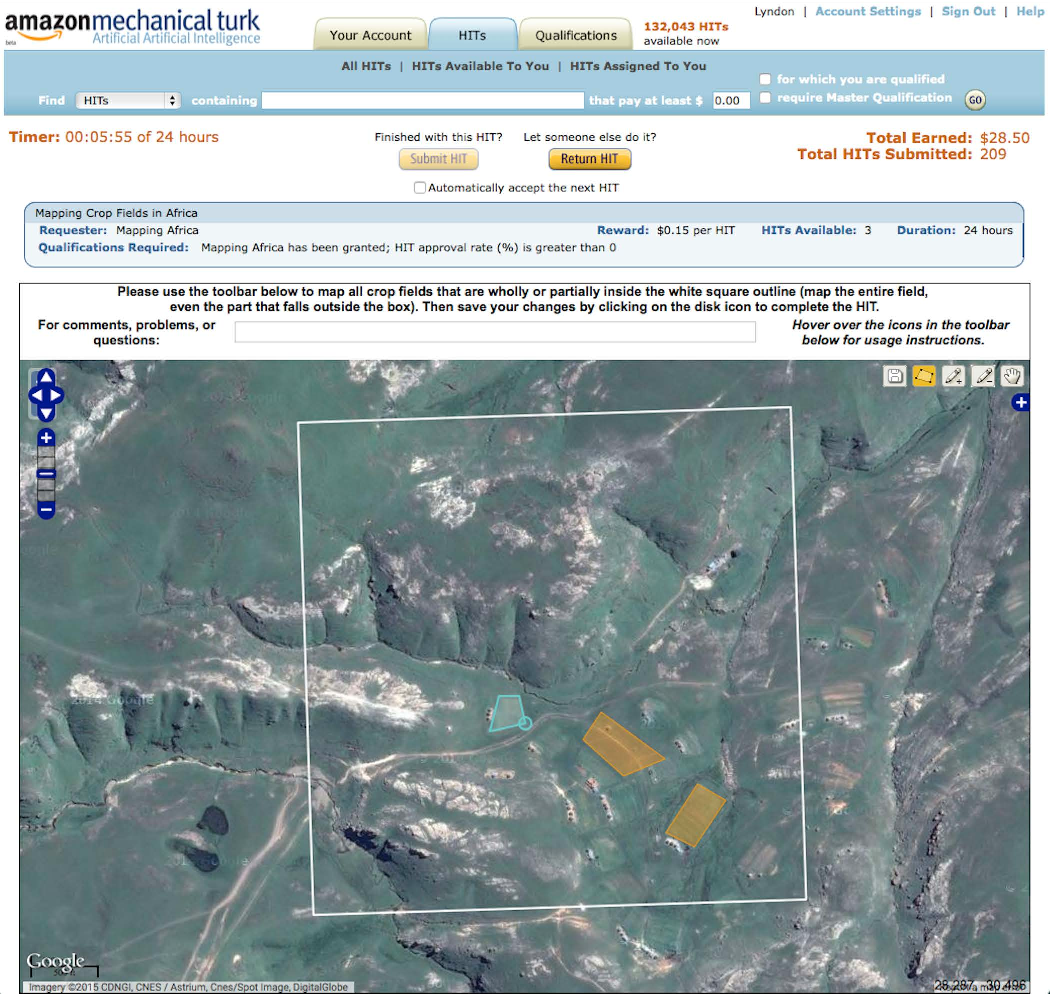
\includegraphics[scale=0.85]{fig3.eps}
    \caption{The DIYlandcover mapping interface within Amazon.com's Mechanical Turk job marketplace. The white square is the KML sampling frame, gold polygons are completed crop field polygons, the blue polygon is a field in the process of being mapped. Mapping controls are in upper right corner of the image frame.}
    \label{default}
  \end{center}
\end{figure}

When the assignment is completed, returned, or abandoned, MT sends an email notification to the main server, where it is retrieved by \emph{ProcessNotifications}, a python process. If the assignment is returned or abandoned, it is marked as unprocessed and returned to the pool of available HITs on MT, and the worker receives no pay. If the assignment was completed, post-processing routines are triggered. 

\subsection{Processing completed assignments}
Several processing steps must be performed before the worker is paid for the completed assignment, which depend on whether the worker created any polygons during the assignment, and whether it was of Q or N type. If the worker created polygons, then the geometries, KML ID, assignment ID, and completion time are stored in the ``user maps'' data table by process \emph{postKML}, which then triggers \emph{mapFix}, a python script that invokes prepair and pprepair \citep{ohori_validation_2012}, which repair the topologies of single and multi-polygons, respectively. This step is essential because hand-digitized polygon data often contain errors, such as self-intersections and unintended overlaps, which can render topologies invalid and cause subsequent spatial analyses (per 3.4) to fail.  The repaired geometries are then inserted into the user maps table.  

Next, the assignment is given a score, which is recorded in the assignment data table. If the assignment was of N type, this score is null;  for Q type, \emph{KMLAccuracyCheck}, an R process, is called to compare the worker's and reference maps, with the score determined by:

\begin{equation}
  \textrm{S} = \beta_1\textrm{C} + \beta_2\textrm{O} + \beta_3\textrm{I}
%  S = \beta_1\left(1 - \frac{abs(n - N)}{max(n, N)}\right) + \beta_2\frac{a}{a + c} + \beta_3\frac{a + b}{a + b + c + d}
\end{equation}

\noindent Where S is overall mapping accuracy, $\beta_1$-$\beta_3$ are user-defined weights, and: 

\begin{equation}
  \textrm{C} = 1 - \frac{\textrm{abs}(\textrm{n} - \textrm{N})}{\textrm{max(n, N)}}
\end{equation}
 
\begin{equation}
  \textrm{O} = \frac{\textrm{a}}{\textrm{a + c}}
\end{equation}

\begin{equation}
 %\textrm{inside} = \left( \frac{\textrm{a + b}}{\textrm{a + b + c + d}}\right)  \vert  \left(\frac{\textrm{a}}{\textrm{a + c}} + \frac{\textrm{d}}{\textrm{b + d}} - 1\right)
 \textrm{I} = \frac{\textrm{A + D}}{\textrm{A + B + C + D}}
\end{equation}

Or: 

\begin{equation}
  \textrm{I} = \left(\frac{\textrm{A}}{\textrm{A + C}} + \frac{\textrm{D}}{\textrm{B + D}}\right)0.5
\end{equation}

\noindent With C being count error, or the agreement between the number of landcover polygons in the worker's maps (n) and in the reference data (N). O measures map agreement for those parts of the worker's and reference polygons that fall \emph{outside} of the KML grid, where a is the area of overlap, and c is the false negative error (i.e. the area of reference field polygons falling outside the grid that the worker failed to map). I measures map accuracy \emph{inside} the KML grid, with A being the grid interior equivalent of a, B the false positive error (i.e. landcover incorrectly labelled by the worker), C the false negative error (landcover area missed by the worker), and D the true negative area (area correctly left unmapped). I can be calculated using standard classification accuracy (Eq. 4), or a variant of the True Skill Statistic \citep[Eq. 5][]{allouche_assessing_2006}, a more stringent measure that corrects for class prevalence, which we compressed to fall between 0 and 1 rather than -1 to 1. The areas of a, c, A, B, C, D are calculated using intersection and difference operations provided by the rgeos library \citep{bivand_rgeos:_2013}, after transforming maps to a projected coordinate system.  

We include the O metric to encourage workers to completely map features intersecting the sampling grid (i.e. either falling entirely within or both within and outside of it), in order to have unbiased estimates of landcover size classes. However, we can only partially assess the accuracy of exterior features because it is impossible to correctly define negative space outside the sample grid, since it is both unbounded and may contain target features that will not be mapped because they do not intersect the grid. An error map showing each of the accuracy assessment components is illustrated in Figure 4.

\begin{figure}[!ht]
  \begin{center}
    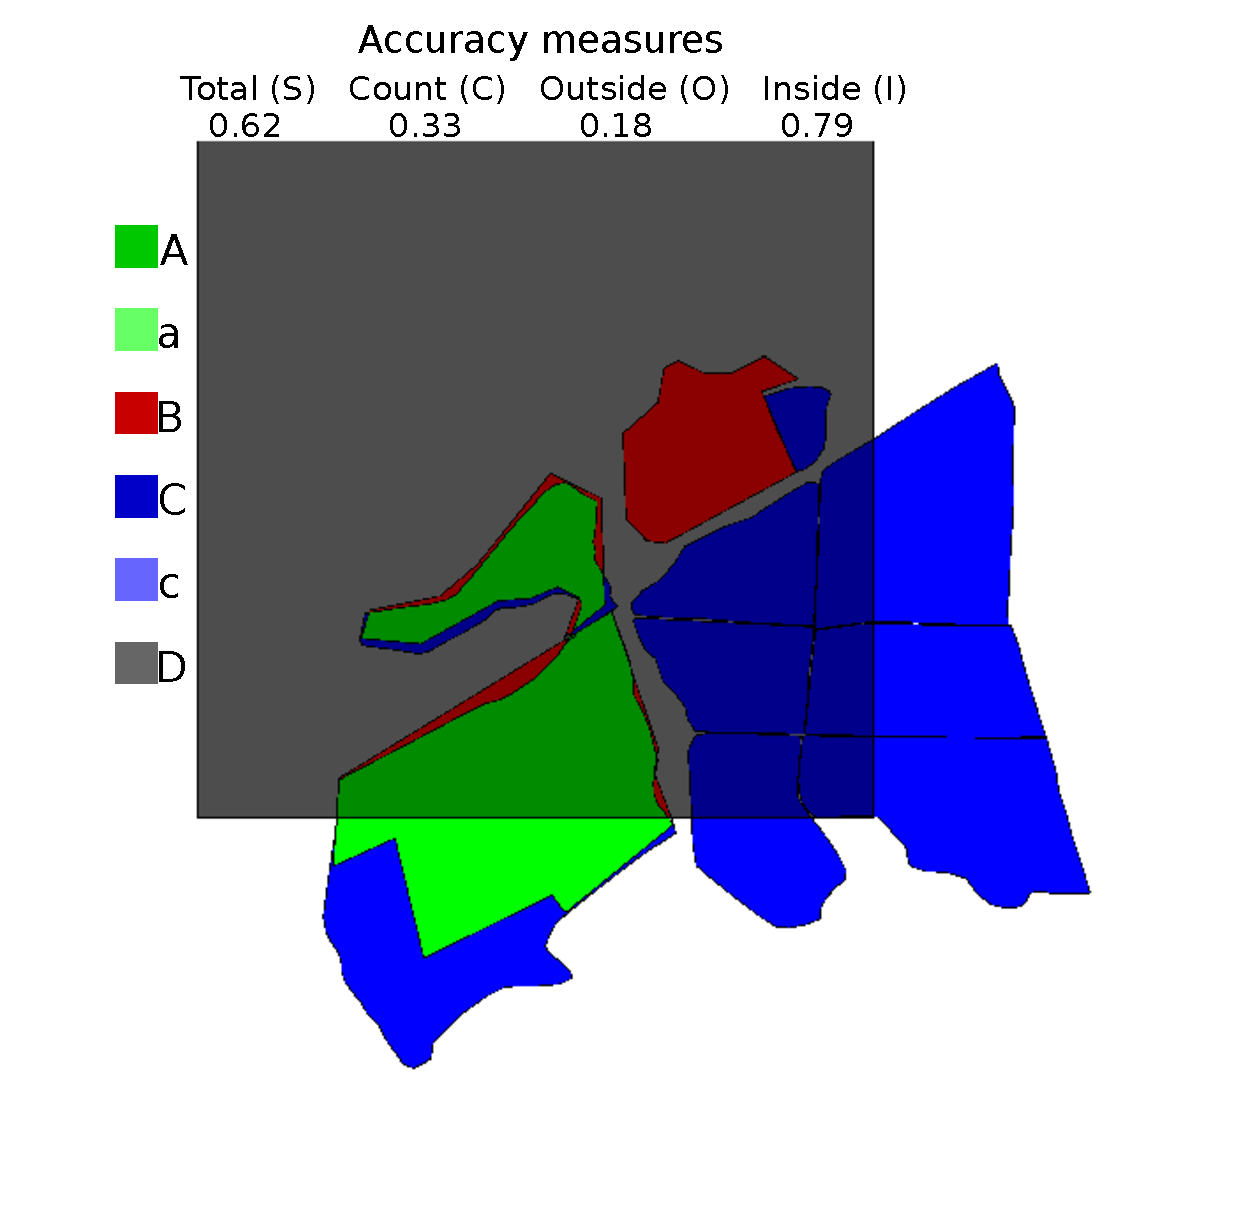
\includegraphics[scale=0.8]{fig4.eps}
    \caption{A graphical illustration of the accuracy assessment algorithm (as applied to cropland maps), providing the resulting scores for overall accuracy (Eq. 1) and count, outside, and inside error (Eqs. 2-5), where each component ranges between 0 (most error) and 1 (no error). The area of each error component is color-coded: A (agreement inside the grid), a (agreement outside), B (false positive error inside the grid), C (false negative inside), c (false negative outside), and D (true negative inside). }
    \label{default}
  \end{center}
\end{figure}

Once the algorithm has run, all accuracy measures (S, C, O, I) are stored in the ``error data'' table, while S is stored in the assignment data table. S is also added to a vector of Q scores for the specific worker (stored in the ``worker data'' table), which is used to calculate a moving average of the worker's recent performance.  If S is above a minimum accuracy threshold, then the assignment is approved. If rejected, then payment is withheld, and a notice is sent to MT where it is added to the worker's system-wide rejection rate. Successive rejections can result in the revocation of mapping qualifications if a worker's \emph{quality} score drops below the accuracy threshold. The quality score is:

\begin{equation}
  \textrm{quality} = \frac{{\textrm{S}_{\textrm{i}} + \textrm{S}_{\textrm{i-1}} + ... + \textrm{S}_\textrm{i-(j-1)}}}{j} - \beta_4\frac{{\textrm{R}_{\textrm{i}} + \textrm{R}_{\textrm{i-1}} + ... + \textrm{R}_\textrm{i-(j-1)}}}{j}
\end{equation}

Where i is the most recent S value calculated, and j the total number of recent S scores to use in calculating a mean S. To minimize assignment selection bias (see 3.3), an additional penalty, the worker's rate of assignments accepted but returned without completing (R, which equals 1 for a return, 0 for a completion), is multiplied by a weight $\beta_4$ and deducted.  

In cases where the worker returns no maps for a Q type assignment, map storage and cleaning does not occur before \emph{KMLAccuracyCheck} is run. In these cases, the C and O scores (Eq. 2 \& 3) reduce to 1 where the reference map has no landcover polygons, or 0 if it does. If the assignment is of N type, it is scored as NULL and added to the assignment data table.  

Unlike the Q type, N assignments are automatically approved, under the logic that the worker's quality score at the time of map creation is indicative of that map's accuracy. The exception to this is N assignments created by a newly qualified worker (see 3.5), which are marked as ``untrusted'' in the assignment data table until that worker completes as many Q assignments as are needed to calculate the moving average accuracy score. Upon assignment approval, \emph{ProcessNotifications} relays a message to MT and the worker is paid (see 3.6) from the Requester's account, and then removes the corresponding HIT from MT. Q sites will be re-created as HITs multiple times, while N sites are mapped just one time.

%\begin{table}[htdp]
%\caption{default}
%\begin{center}
%\begin{tabular}{|c|c|}

%\end{tabular}
%\end{center}
%\label{default}
%\end{table}%

\subsection{Worker qualification and payments}
All workers performing mapping assignments must first be qualified, which is treated as a special case of Q type assignments. MT evaluates the qualification status of each worker attempting to access a DIYlandcover HIT. If the worker is not qualified, a link to a training module is presented on the MT interface. The module, which is hosted on the main server, is managed by \emph{trainingframe}, a python process, which issues each new trainee a unique training ID. The trainee first watches video tutorials explaining the project and its mapping rules, and is then required to map several training sites, the accuracy of which is assessed by \emph{KMLAccuracyCheck}. Trainees must map each site to the minimum accuracy standard, but are given unlimited chances to do so. A separate set of tables mirroring those used for collecting map, assignment, worker, and error data is used to record training data. Once a worker successfully completes all training sites, a qualification request is posted on MT.  A daemon, \emph{process\_qualifications\_requests}, polls MT at specified intervals, collects these requests together with associated worker and training IDs, examines for each worker whether all training sites were completed successfully, and, if so, adds the trainee's worker ID to the worker data table, sets the qualification status to true, then sends a notice to MT that the worker is now qualified. Candidate workers who fail to pass all training sites, or workers whose qualifications are revoked due to poor accuracy (see 3.4), can repeat the training to qualify/re-qualify. 

%Each worker who attempts to access a The ID of each worker who attempts to access a DIYlandcover HIT is compared against the worker data table by\emph{ProcessNotifications}. If the worker's ID is not found, a link to a training module is presented on the MT interface.

Upon qualification, workers are paid a small bonus, and can begin mapping assignments. Workers are paid a flat rate for approved assignments. To incentivize worker performance, DIYlandcover also allows bonus payments to be made based on the worker's accuracy score. If implemented, the bonus algorithm, managed by \emph{ProcessNotifications}, pays an extra per assignment amount if the worker's quality score exceeds certain thresholds.

\section{Applying DIYlandcover to map South African crop fields}
We examined the capabilities of DIYlandcover by applying it to map crop field boundaries in South Africa. South Africa was a convenient test case because it cropland was already mapped \citep[see section 2;][]{geoterraimage_south_2008} using similar methods, providing both an objective means for evaluating DIYlandcover's performance, and a readily adaptable source of reference maps. Furthermore, South Africa's diversity of agricultural systems are representative of the image interpretation challenges facing workers. This mix ranges from hard to detect communal and smallholder agriculture, to more easily discerned industrial fields \citep{hardy_rainfed_2011}. South Africa also provides the test site for the \href{http://mappingafrica.princeton.edu}{Mapping Africa} project, which aims to create high quality cropland maps for sub-Saharan Africa. 

\subsection{Mapping set-up}
We created a 1X1 km, Albers Equal Area Conic-projected sampling grid for South Africa, and used logistic regression to model the probability of cropland presence throughout the country. Equally sized random draws of points selected inside and outside GTI field boundary polygons provided the positive and negative responses of the dependent variable, while predictors were derived from gridded rainfall and elevation data and a map of protected areas \citep[for further details on these variables see][]{estes_comparing_2013,estes_using_2014}. The resulting probability was divided into quartiles, which provided the weights used by \emph{KMLGenerate}.

For Q sites, we used the modeled cropland probability categories to draw a random select 609 grid cells (0.05\% of South Africa's area), providing a representative sample of South Africa weighted towards agricultural areas. We intersected these with the GTI polygons to create the associated Q data tables (3.1). These polygons were then further edited to make the Q maps consistent with imagery in the Google Maps API, and to conform with the specific mapping rules that we set for workers (Table 1). Workers were asked to map sites where crop fields were actively or very recently (i.e. within the past 2-3 years) used for arable agriculture. This category of agriculture takes many forms in South Africa (see Appendix S1 for an illustration), ranging from large, clearly defined, commercial fields to less geometrically distinct smallholder fields, which often contain trees and mixed crops. Long term fallows, tree crops (orchards, commercial afforestation), and non-agricultural areas were left unmapped. In cases of uncertainty (e.g. the worker had trouble telling whether the field was active or abandoned), workers were asked to map every second field. On top of the high variability in arable fields, narrowing the mappers' focus actually made the task more challenging, because the agricultural types described in Table 1 often look similar, which increases the risk of both false positive and false negative errors. For instance, it is often difficult to tell whether a field is active or abandoned, while young orchards or recently cleared forest compartments can be mistaken for arable fields. In all these examples, field boundaries tend to be clearly visible, thus more inclusive mapping rules would likely reduce both types of error. 

\begin{table}[htdp]
  \caption{Rules for mapping crop fields in the South Africa-focused application of DIYlandcover. Workers were asked to map only currently active (i.e. farmed within the past 2-3 years) annual crop fields, and to not delineate other agricultural types.}
   \begin{center}  
   \begin{tabular}{l|l}
      \hline
      \textbf{Feature type} & \textbf{Action} \\
      \hline\hline
      No cropland visible & Don't map \\
      Active annual crop field & Map \\
      Fallow crop field & Don't map \\
      Unsure if active crop fields & Map every second feature \\
      Permanent tree crops (orchards/plantations) & Don't map \\
      Improved pastures & Don't map \\
     \hline
  \end{tabular}
  \end{center}
  \label{default}
\end{table}%

The system was set to make random draws of 500 N sites from the master grid each time the number of N sites available for mapping fell below 500 (3.1), in order to ensure that no system latency occurred as the system selected new mapping locations. At least 10 HITs, 80\% N and 20\% Q, were maintained on MT at any given time, with the system polling MT every 10 seconds to see if new HITs were needed (3.2). This relatively low number allowed rapid cycling of HITs through MT, while the ratio of N:Q HITs ensured that worker accuracy was assessed (3.4) frequently during the trial (once in every five assignments). 

The accuracy algorithms (Eq. 1) $\beta$ terms were set as 0.1, 0.2, and 0.7 for the C (Eq. 2), O (Eq. 3), and I terms (here Eq. 4). We selected a low weight for C because determining the boundaries of individual fields from overhead imagery is fairly subjective, even for expert observers, and we did not want to unduly penalize workers for a difference in judgement, yet we also wanted to discourage rapid mapping that erased boundaries between clearly distinct fields. We gave O a slightly larger weight to stress the importance of completed fields that extended outside the sample grid, but a larger weight would give the worker too much credit for cases where no fields intersected the grid. The I term was weighted most heavily because it is the only place where workers' abilities to correctly distinguish null space can be assessed.  We used the same weights to assess assignments within the 8-site training module.       

Payment was set at \$0.15 per assignment. A four-tier bonus payment algorithm was also written into logic. We did not implement this logic in our initial trial, in order to first assess whether the base rate would allow workers to achieve our target wage of \$8-10 hour$^{-1}$, but we evaluated the cost implications of bonus payments set to \$0.01, \$0.02, \$0.03, and \$0.05 for worker quality scores exceeding 0.85, 0.95, 0.975, or 0.99, respectively. 

\subsection{Trial results}
The Mapping Africa trial ran on Mechanical Turk for 26.4 hours between October 2-3, 2013, resulting in 945 mapping assignments, of which 882 were approved, 10 were rejected (due to failing accuracy scores), and 53 were not completed (i.e. returned or abandoned).  A total of 707 N sites with 216 (31\%) containing worker-delineated polygons were mapped, as well as 185 Q sites, with 65 (35\%) having fields (Fig. 5). 

\begin{figure}[!ht]
  \begin{center}
    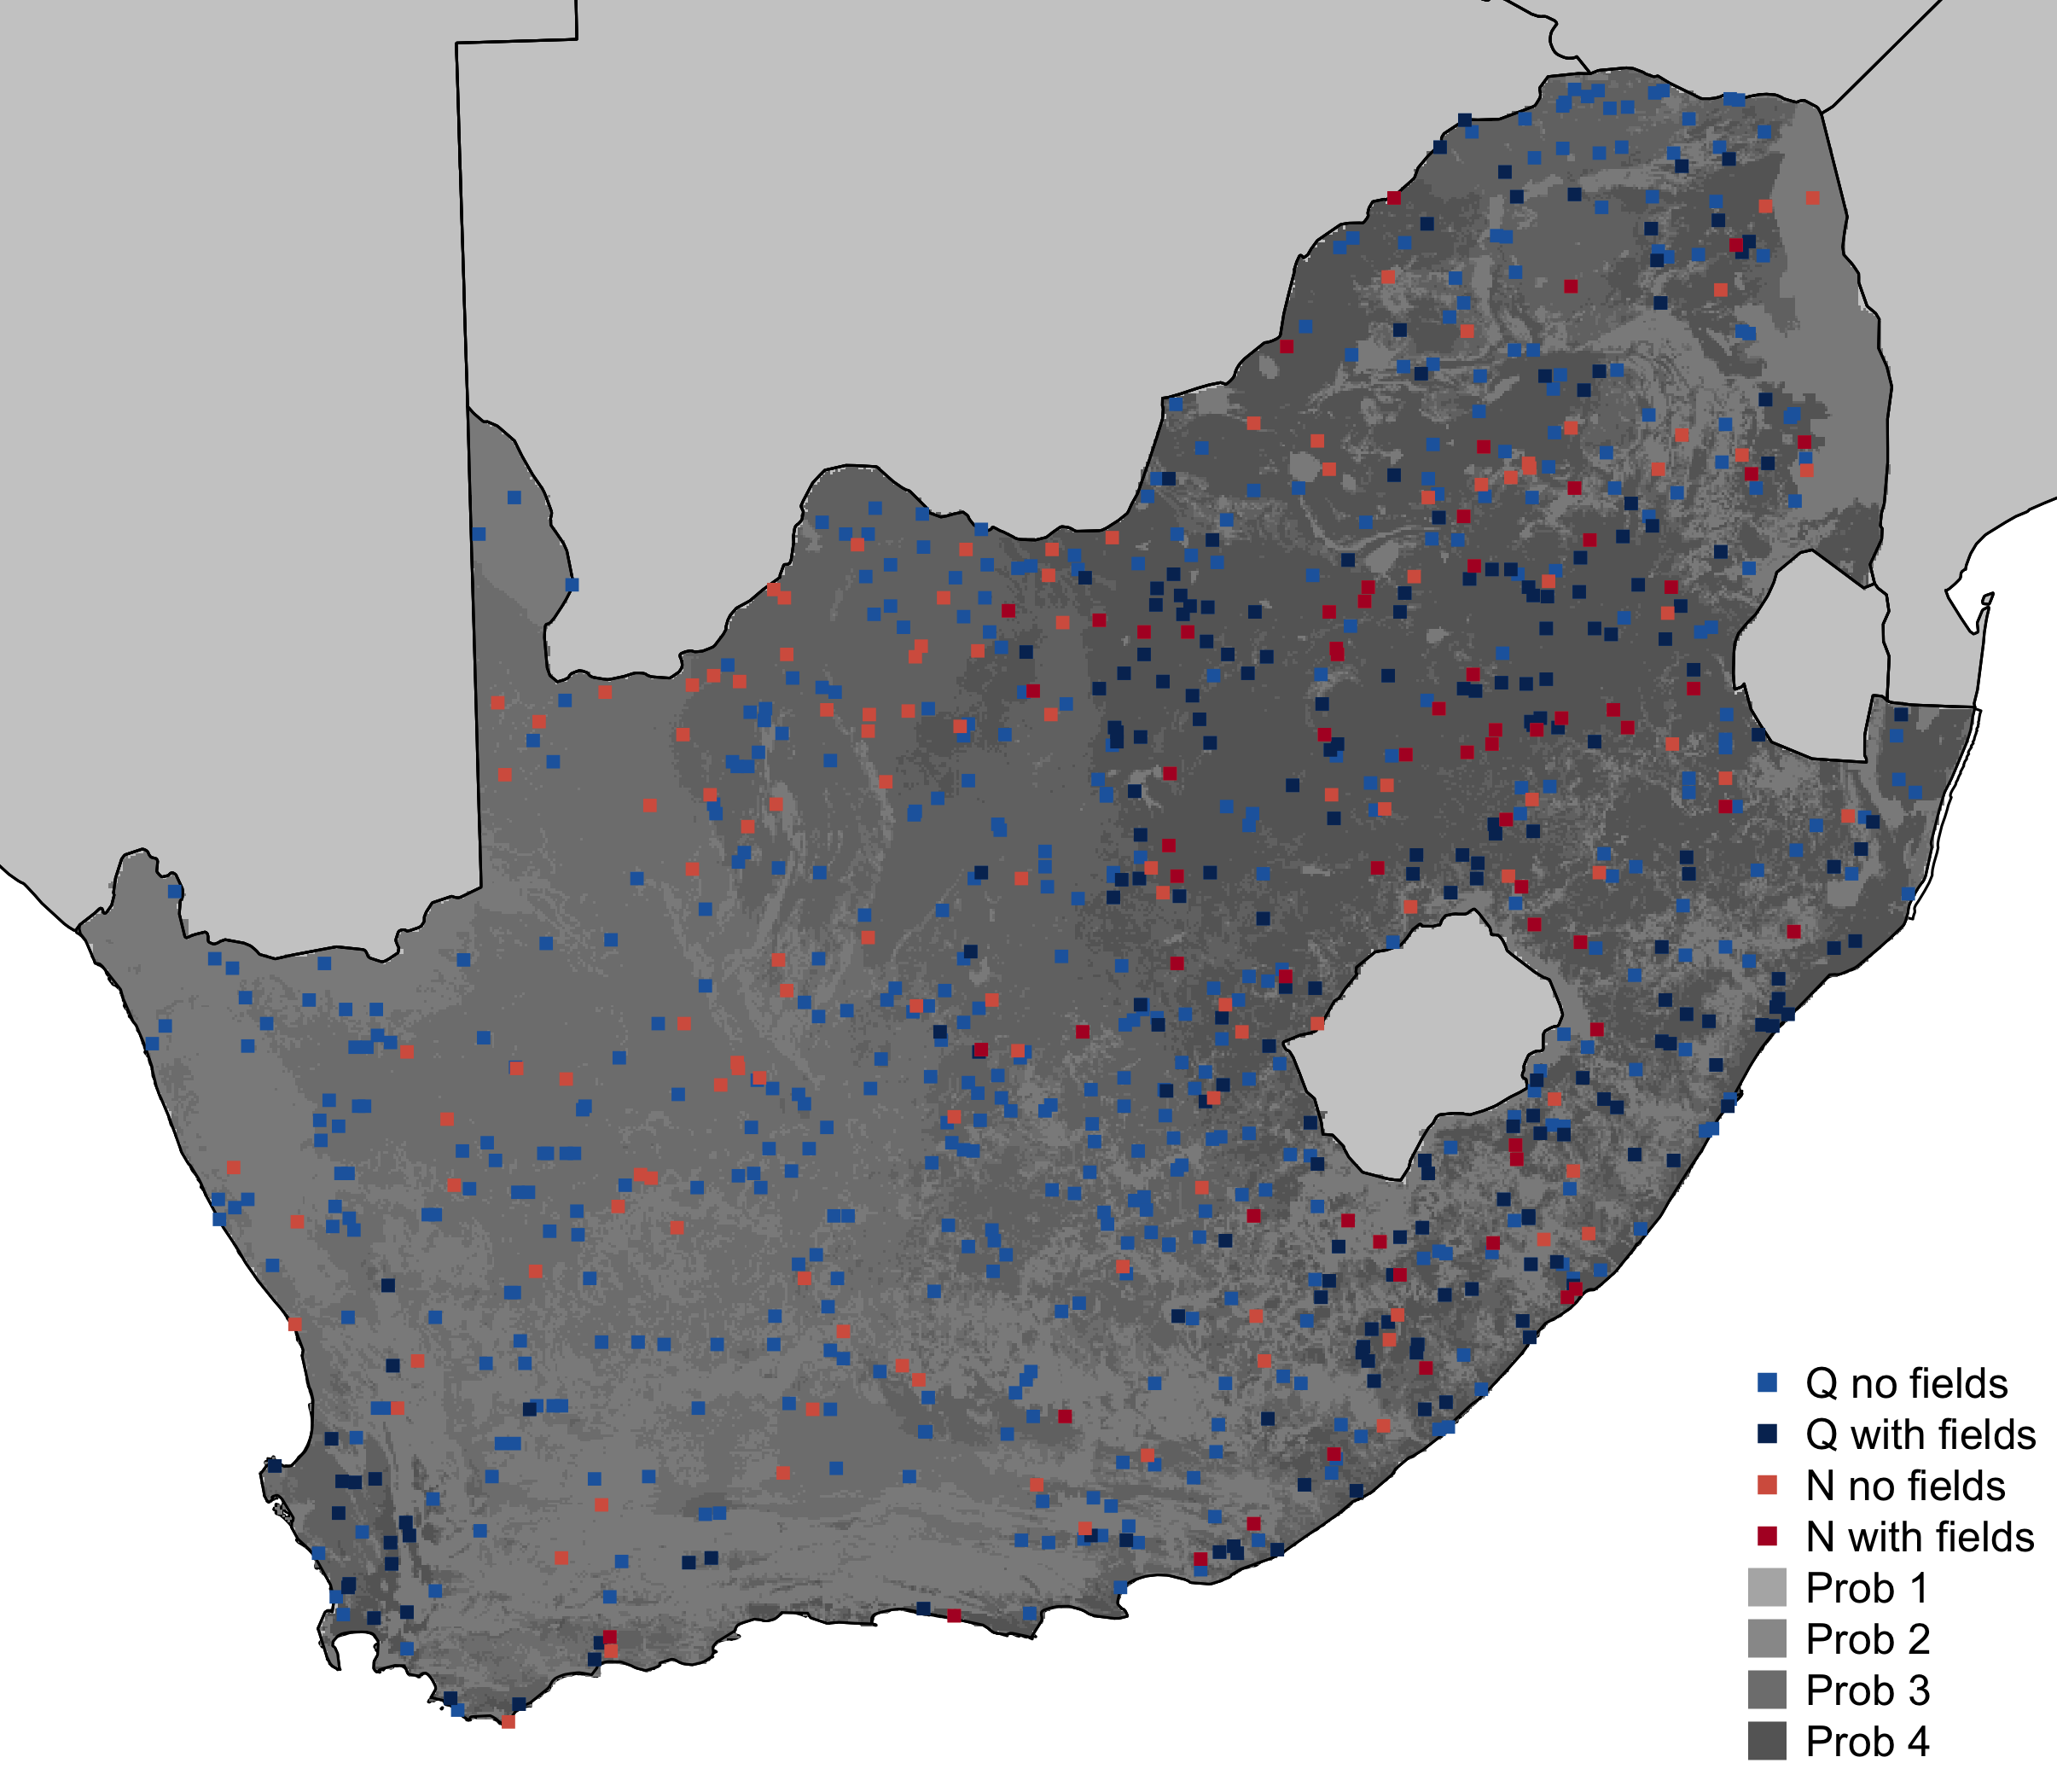
\includegraphics[scale=0.7]{fig5.eps}
    \caption{A map of DIYlandcover trial results over South Africa, showing the distribution of mapped sites, color-coded according to their assignment type (Q or N) and whether they contained worker-mapped crop field boundary polygons. The grey shading indicates the four-category weighting derived from a logistic regression model of cropland occurrence.}
    \label{default}
  \end{center}
\end{figure}

These sites were mapped by 15 different workers, from a pool of 18 who passed the initial qualification test. A further 18 took the qualification test but failed to pass. The distribution of mapping effort was highly skewed, with three workers completing 65\% of the total assignments (Fig. 6A).  The average Q:N assignment ratio for each worker was 18\%, but there was high variability among workers who completed less than 50 assignments (Fig. 6A). The mean accuracy assessed across all Q sites (using Eq. 1 with Eq. 4) was 0.91 (out of 1), but Q sites containing fields were mapped with lower overall accuracy (0.79) than sites without fields (0.97; Fig. 6B). Using just the inside component of the score (Equation 4), accuracy was higher for sites with fields (0.89 with fields versus 0.99 without). To understand these accuracy discrepancies more fully,  the number of polygon vertices in the reference polygons can be used as proxy for cropland complexity, and thus assignment difficulty.  Worker accuracy declined significantly, albeit weakly (p$<$0.048), in relation to this complexity (Fig. 6C). Worker effort also declined strongly as a function of map complexity (Fig. 6D); the more fields there were to map---or the more intricate their boundaries---the fewer vertices placed by workers, presumably to minimize mapping time. This reduction in effort may partially explain the increased error. 

\begin{figure}[!ht]
  \begin{center}
    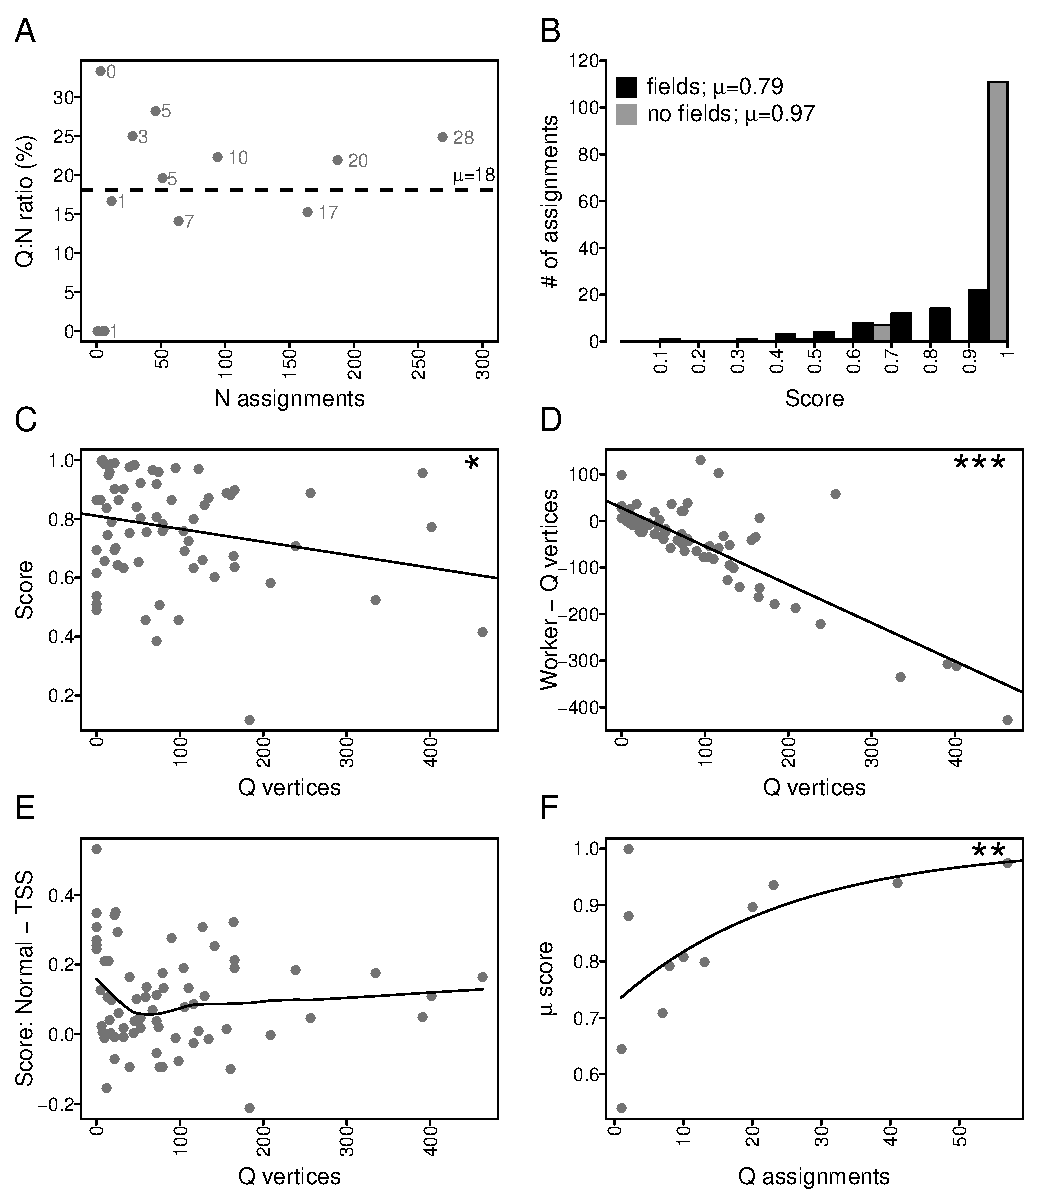
\includegraphics[scale=0.66]{fig6.eps}
    \caption{Results from initial DIYlandcover trial, including A) the total number of completed assignments per worker versus the ratio of Q to N type assignments (values in grey next to points represent the percent of total assignments); B) the distribution of accuracy scores segregated by assignment type (black bars = Q type, grey bars = N type); the number of vertices in reference map polygons versus C) accuracy score, D) the difference between the number of vertices in workers' and reference map polygons, and E) the difference between accuracy scores calculated using Equation 4 or Equation 5 (the True Skill Statistic); F) the number of Q assignments completed by each worker versus worker mean accuracy score. Significance of regression fits in C, D, F are:  $\ast$p$<$0.05; $\ast$$\ast$p$<$0.01; $\ast$$\ast$$\ast$p$<$0.001. C and D are linear models, F is asymptotic regression.} 
    \label{default}
  \end{center}
\end{figure}

Replacing Equation 4 with Equation 5 (the True Skill Statistic; TSS), which corrects for class prevalance  \citep{allouche_assessing_2006}, to calculate map score (Eq. 1) removed the significant negative relationship between map score and complexity (F-statistic: 0.98; p$<$0.32). At sites with only a few fields, which are both less complex and typically having a much higher share of non-cropped than cropped area, Eq. 4 was more lenient than at more complex sites, because the worker received proportionally more credit for ``mapping'' the uncropped space.  This tendency is seen in Fig. 6E, which shows that map scores calculated using Equation 4 were generally higher than those assessed using Equation 5; for sites with fields, scores were on average 0.1 higher, and up to 0.14 greater where fields were relatively simple (i.e. where truth maps had $<$25-50 vertices, indicating both low complexity and small areas).

Accuracy appears to improve with experience, as workers' average accuracy scores increased in proportion to the number of Q assignments completed. Accuracy gains increased rapidly below 20-25 completed Q assignments, after which they leveled out between 0.9 and 1 (Fig. 6F).  

%N sites per worker
%Accuracy
%Accuracy per worker
%Accuracy as function of vertex density 
%Accuracy as function of time/experience

We paid \$132.30 to workers for the 882 approved assignments, with a total cost to the project of \$145.53 after accounting for Amazon.com's 10\% Requester surcharge. Of this, \$28.88 was paid for the 175 approved Q assignments and \$116.66 for the 707 N assignments.  Our post-hoc application of the bonus algorithm, which requires workers to complete at least five Q assignments (8 of 15 met this requirement), would have added \$21.89 (15\%) to the trial's cost. 

To examine the effective worker wage (i.e. the amount the worker would expect at these rates assuming constant, uninterrupted work), we divided total pay by the mean assignment duration, calculated as the difference between assignment acceptance and completion times. Since workers could accept assignments without immediately completing them (maximum assignment duration was 24 hours), we could not precisely measure mapping time. However, our experience suggests that the most complicated sites require $<$30 minutes of mapping effort, thus we excluded any assignments taking longer than this. The resulting average effective wage was \$10.80 hr$^{-1}$ across all sites, but just \$3.26 hr$^{-1}$ for sites having fields compared to \$13.40 hr$^{-1}$ for sites without fields.  Factoring in bonus payments, these would have been \$11.65 overall and \$3.55 and \$14.53 for sites with and without fields (Table 2). 

The flat rate cost to map a single square kilometer was \$0.165, including the cost of accuracy assessment and Amazon.com's fees, or \$0.19 had we included bonus payments. 

%At these rates, the cost of mapping South Africa in its entirety (1,219,095 1 km$^2$ cells) would be \$201,151-231,407, or \$3.4-3.9 million for all of non-Saharan Africa (20.8 million km$^2$). 

\subsection{Estimating the costs of scaling up}
We used the time and cost results from the trial to estimate the potential costs of mapping larger regions, in terms of worker payments and total mapping time, using two different payment models. One models used fixed base rates (as in our trial), the other variable rates linked to potential mapping effort, and in each case we tested two different levels of payments: for the fixed case we used rates of \$0.15 and \$0.05\footnote{Estimated as the approximate difference between US and South African minimum wages, http://businesstech.co.za/news/international/87614/minimum-wage-in-south-africa-vs-the-world/}; for the variable rate, payments rates were set using the following formula: 

\begin{equation}
\textrm{R} = \$0.01 + (\sum_{\textrm{w}=1}^{\textrm{n}} - 1)\textrm{I}   
\end{equation}

Where R is the rate, w is a categorical weight derived from a map of cropland probability, and I is an increment, set here to \$0.07 and \$0.023 for the higher and lower pay models, respectively (see Appendix S3 for methods).  For the cropland weights, we converted the GeoWiki 1 km$^2$ cropland percentage map \citep{fritz_mapping_2015} into a 10 category map (where 1 = 0-10\% cropland and 10 = 90-100\% cropland). This map provided a more finely resolved set of weights than our four category map, and covered the entire continent. Since cropland percentages correlate positively with field area and number (albeit with area), these weights also provided a proxy measure for likely mapping effort. We confirmed this assumption by extracting the new weights corresponding to the areas mapped, and used them in a least squares regression to model workers' observed mapping times (R$^2$=0.1, p$<$0.0001; Appendix S3). The map weights were extracted into a reordered vector using DIYlandcover's weighted random sampling protocol (see 3.1), and then used with Equation 7 to assign payments for each site. We added the trial mean bonus rate (\$0.023) onto these payments (and to the fixed pay rates), then calculated the cumulative cost for mapping all 29,924,000 km$^2$ of Africa for each pay model, multiplied by 1.4 to represent 1) an additional 10\% of mapping effort for quality assessment, and 2) administrative costs of 30\%. 

To estimate the total time required to map the continent, we used the predicted mapping times resulting from the regression model. The model was run 1000 times on random subsets of the data to obtain prediction uncertainties for each weight level, from which the mean, 2.5\textsuperscript{th}, and 97.5\textsuperscript{th} percentile values were extracted. These predicted time values were assigned to their corresponding weights in the reordered weights vector, from which mean, upper, and lower estimates of cumulative mapping hours were calculated (Appendix S3). We then created three hypothetical models of worker involvement, in which either 100, 250, or 500 workers, each mapping one hour per day, undertook the work, and used the resulting daily total mapping hours to convert the cumulative mapping time into estimates of how long it would take to map the entire continent (in years). 

The cost model results show that variable pay rates would be considerably more efficient than fixed rate methods (Figure 7, left panel). At the trial pay rates, it would cost \$7.23 million to map the entire continent, whereas it would cost just \$3.47 million using a variable pay rate, which is not much higher than \$3.04 million that would be required if pay was at the lower fixed rate. Applying the cheaper variable rate scheme, the cost would be just \$2.07 million to map all of Africa. Applying these alternate payments rates for the sites mapped during the trial reveals that variable rates would produce overall effective wages comparable to fixed rates, while paying nearly 50\% higher, on average, for mapping sites with fields (Table 3).  

Total mapping time estimates vary widely according to the number of workers involved, ranging from more than 19 years to map the whole continent with just 100 workers involved (i.e. 100 mapping hours per day) at the upper confidence limits of mapping time, to 1.2 - 3.8 years (mean = 1.9 years) if 500 workers map.  

\begin{figure}[!ht]
  \begin{center}
    \includegraphics[scale=0.78]{fig7.eps}
    \vspace{-1cm}
    \caption{Several estimates of the cumulative cost (left) and time (right) of using DIYlandcover to map cropland throughout Africa. Cost estimates are based on either fixed (solid line) or variable (dashed line) rates, using higher (blue) and lower (green) cost models for each case. The cumulative mapping time is calculated in years, based on three different levels of worker involvement (100 [red], 250 [blue], and 100 [green] workers, each mapping for 1 hour/day). Solid lines indicate regression-predicted means, dashed lines the upper and lower confidence bounds for each model. } 
    \label{default}
  \end{center}
\end{figure}

\begin{table}[htdp]
  \caption{Effective wages for workers (in \$ hr$^{-1}$) under two fixed and two variable payment schemes, calculated as overall averages and for mapping sites with and without fields, and including mean bonus rates. }
%   \begin{center}  
%   \begin{tabular}{l|l}
%      \hline
  \centering
  \begin{tabular}{rrrr}
    \hline
    Payment method  & Overall & With fields & Without fields \\ 
   \hline
    Fixed high & 11.65 & 3.55 & 14.53 \\ 
    Variable high & 10.16 & 5.19 & 12.16 \\ 
    Fixed low & 4.44 & 1.38 & 5.59 \\ 
    Variable low & 4.43 & 2.07 & 5.39 \\ 
   \hline
  \end{tabular}
\end{table}

\section{Discussion}
The initial trial demonstrates that DIYlandcover can be an effective platform for generating high quality maps of discrete landcover types. This quality is attributable to humans' superior ability to recognize objects in patterns in noisy backgrounds, and is the reason why expert image interpretation is a key component of training and assessing existing landcover mapping algorithms \citep[e.g.][]{fritz_cropland_2011,fritz_geo-wiki:_2012,hansen_high-resolution_2013}. Here we found that workers with less than 24 hours of mapping experience were able to map cropland with 91\% accuracy. Although accuracy and mapping precision decreased when sites contained crop fields, and in proportion to the complexity of those fields (Fig. 6), the overall accuracy was higher than the latest generation landcover dataset of comparable resolution \citep[82\%;][]{fritz_mapping_2015}, and was close to that achieved by GTI's trained workers. Compared to GTI's performance at sites with fields, using the most comparable accuracy metric (Equation 4), DIYlandcover showed similar performance--even though the score was 6\% lower than GTI's 95\% (see Appendix S1)--because GTI mapped using a more inclusive set of rules, thereby reducing error rates, and DIYlandcover's accuracy algorithms are more precise than the one used to assess GTI performance (see Fig. 6B and Appendix S1). The positive relationship we see between worker experience and score (Fig. 6F) also suggests that DIYlandcover's accuracy improves with time, and we expect that the implementation of bonus payments for performance will also improve mapping skill. These latter two points will need to be evaluated after a lengthier period of production, as does the affect of the different accuracy component weights (Eq. 1) in terms of influencing worker--and thus system--performance. 

The trial also suggested that DIYlandcover has the potential to generate map data relatively rapidly, given an adequate number of workers (Figure 7). With 500 workers each contributing one hour of work per day, we estimate that all of Africa could potentially be mapped in approximately 1.9 years, which is roughly six month faster than the time needed to create GTI's map for South Africa. It is not unreasonable to think that this level of worker involvement is feasible on a for-pay crowdsourcing platform, particularly given the payment rates we applied, which were substantially greater than the \$2 hr$^{-1}$ received by Mechanical Turk workers \citep{marvit_how_2014}. 

Our cost assessment (Fig. 7) indicates that linking pay to cover occurrence probabilities--and site selection to a finer gradation of weights--could greatly reduce the overall costs of ``wall-to-wall'' mapping, while maintaining fair worker wages. Although \$3 million is a significant amount of money, we argue that it would be a fairly cheap price to pay for a vector-based map of individual crop fields covering all of Africa. The overall mapping costs could be reduced to \$2 million if payments are made at the lower rates we assessed. We do not advise this approach when running the software on MT, as the worker base is primarily in the US given Amazon's fairly strict payment rules\footnote{www.mturk.com/mturk/help?helpPage=worker}, and because there is growing concern about the exploitative nature of crowdsourcing \citep{marvit_how_2014}. However, it may be possible to pay \emph{fairly} at lower rates if DIYlandcover is ported to job sites where workers can access it from countries with lower prevailing wages. For instance, in our example, had we been able to enlist workers in South Africa, where the exchange rate favors the dollar, we could have paid less and had mapping undertaken by workers who were familiar with those landscapes.   

Other costs related to system development time could also be reduced, particularly with respect to generating reference maps. Our trial reference maps took several weeks to digitize, and were based on the judgement of a few people. A third type of mapping HIT, one that allows repeated mapping by multiple workers, would help mitigate these problems of cost and subjectivity. The resulting maps could be combined to create a more robust ``truth'' based on between-worker agreement, as illustrated by the combined maps from the eight qualification sites used in the trial (Fig. 7). This approach could greatly minimize the time required to develop reference data, and we suspect that the consensus maps of many workers (which could be weighted based on worker quality scores) will be more accurate than those of one or two experts (the last assumption must be verified against field-collected boundary data). Another advantage of this approach, which will be incorporated in the next update of DIYlandcover, is that the quality assessment protocol would essentially become a form of peer review. 

\begin{figure}[!ht]
  \begin{center}
    \includegraphics[scale=0.78]{fig8.eps}
    \caption{The eight sites used in the South Africa trial qualification test. Columns 1 and 3 show the unmapped imagery; columns 2 and 4 display the combined maps of all 19 trainees.  Map colors indicate the fraction of trainee maps that overlap. } 
    \label{default}
  \end{center}
\end{figure}

Of course, the costs and necessary mapping time assessed here may still be too much for many users who need spatially comprehensive, large area landcover maps. To reduce costs, DIYlandcover could be ported to a server that supports voluntary crowdsourcing efforts, similar to the Geo-Wiki project \citep{fritz_geo-wiki:_2012}, but this would not address the problem of longer mapping times. An alternative, more advanced, application would be to use DIYlandcover to train and test newer computer vision approaches for mapping noisy landcover types, such as smallholder crop fields \citep[e.g.][]{debats_generalized_2015}. In this case, DIYlandcover would work iteratively with the algorithm until an acceptable level of accuracy is achieved, with site selection weighted towards areas of greatest classification error after each step. This approach could strike the best balance between cost, mapping speed, and accuracy, as it would harness the complementary strengths of human (more effective at recognizing patterns in noisy RGB or black and white images) and computer image classifiers (able to extract patterns in high dimensional data, such as multispectral imagery, which are hard for humans to interpret).  An alternative possibility for this use case---where DIYlandcover validates broader-scale methods---would be test and refine the judgement-based size class estimates created under the Geo-Wiki project \citep{fritz_mapping_2015}. DIYlandcover is highly complementary to this methodology, given its emphasis on precisely measuring landcover geometries.   

Beyond the questions of accuracy, cost, and time, the geometric detail captured by vector boundaries is a key data dimension that is lacking from current landcover products, and difficult to obtain from automated approaches. It is this capability to map individual features that may appeal to the broadest range of potential users, as geometry data provide information on a number of important social, economic, and environmental processes. For instance, crop field sizes can be effective predictors of agricultural economic metrics, and as such development-oriented agencies may be significantly interested in using this tool to generate these data \citep{fritz_mapping_2015}. Alternatively, conservationists wanting to identify habitat fragments to protect may be interested in more precise boundary data, as patch geometry correlate with extinction \citep{laurance_fate_2011} and thus conservation values. Other potential uses include mapping buildings, burn scars, water holes, and termite mounds, to name a few.  

\section*{Acknowledgements}
This work was supported by funds from the Princeton Environmental Institute Grand Challenges program, the NASA New Investigator Program (NNX15AC64G), and the National Science Foundation (SES-1360463 and BCS-1026776).   

\section*{Supplementary materials}
Supplementary methods are presented in Appendix S1; Supporting figures S1 and S2 are found in AppendixS2; Appendix S2 contains the R code used to analyze trial results and create related figures. 

%\label{}

%% The Appendices part is started with the command \appendix;
%% appendix sections are then done as normal sections
%% \appendix

%% \section{}
%% \label{}

%% If you have bibdatabase file and want bibtex to generate the
%% bibitems, please use
%%
\section*{References}
\bibliographystyle{elsarticle-harv2} 
\bibliography{main}

%% else use the following coding to input the bibitems directly in the
%% TeX file.

%\begin{thebibliography}{00}
%
%%% \bibitem[Author(year)]{label}
%%% Text of bibliographic item
%
%\bibitem[ ()]{}
%
%\end{thebibliography}
\end{document}

\endinput
%%
%% End of file `elsarticle-template-harv.tex'.
